\chapter[Two-Phase Stokes Flow FEM]
{\sc Finite Element Approximation for Two-Phase Stokes Flow}\label{ch:stokes}
We now propose a novel finite element approximation for incompressible
two-phase Stokes flow that naturally avoids spurious velocities. Our scheme uses
a fitted approach with piecewise linear parametric finite elements to describe
the moving discrete interface and employs standard velocity and pressure finite
element spaces in the bulk. This chapter is extensively based on a paper we
wrote, see \cite{stokesfitted}.

The chapter is organised as follows: in \S\ref{sec:stokes_model} we state the
mathematical model for the incompressible two-phase Stokes flow; in
\S\ref{sec:stokes_weak} we derive the weak formulation on which our finite
element approximation is going to be based; in \S\ref{sec:stokes_energy} we show
an energy bound and the volume conservation for the weak problem; in
\S\ref{sec:stokes_fem} we present our fitted finite element discretization; in
\S\ref{sec:stokes_fitted_unfitted} we outline the main differences between a
fitted and an unfitted approach; in \S\ref{sec:stokes_existence} we prove the
existence and uniqueness of the discrete approximation; in
\S\ref{sec:stokes_stability} we demonstrate that our scheme is unconditionally
stable; in \S\ref{sec:stokes_stationary_solution} we show some properties of
stationary solutions which will be investigated in the numerical experiments; in
\S\ref{sec:stokes_semi_fem} we investigate the equidistribution property and the
volume conservation of a semidiscrete variant of the scheme; in
\S\ref{sec:stokes_algebraic_system} we describe the arising linear systems; in
\S\ref{sec:stokes_solution_method} we explain the Schur complement approach used
to solve the algebraic system and the preconditioners adopted; in
\S\ref{sec:stokes_smoothing} we discuss the mesh generation process together
with the smoothing and remeshing procedures used to preserve the mesh quality.

\section{Mathematical model}\label{sec:stokes_model}
We consider two-phase Stokes flow in a given domain $\Omega\subset\R^d$, where
$d=2$ or $d=3$. As already described in \S\ref{sec:free_boundary_flows},
the domain $\Omega$ contains two different immiscible, incompressible, viscous
fluids (liquid-liquid or liquid-gas) which for all $t\in[0,T]$ occupy time
dependent regions $\Omega_+(t)$ and
$\Omega_-(t):=\Omega\setminus\overline{\Omega}_+(t)$ and which are separated by
an interface $(\Gamma(t))_{t\in[0,T]}$, $\Gamma(t)\subset\Omega$. In this
thesis, we always treat interfaces formed by closed hypersurfaces, as
illustrated in Figure~\ref{fig:two_phase_sketch} for dimension $d=2$.

The interface $\Gamma(t)$ is described with the same technique used in the
approximation of mean curvature flow and surface diffusion, see
Chapter~\ref{ch:geometric_pdes}. More precisely, we use a front tracking
approach, see \S\ref{sec:front_tracking_approach}, which parametrize the
unknown interface $\Gamma(t)$ as $\vec x(\cdot,t):\Upsilon\to\R^d$ where
$\Upsilon\subset\R^d$ is a given reference manifold such that $\Gamma(t) = \vec
x(\Upsilon,t)$. We always require that the evolving hypersurface is sufficiently
smooth and without boundary. Therefore, the velocity $\V$ of $\Gamma(t)$ is
defined by the equation (\ref{eq:V}) which we report here for the benefit of
the reader
\begin{equation*}
\V(\vec z, t) := \vec x_t(\vec q, t) \quad
\forall\ \vec z = \vec x(\vec q,t) \in \Gamma(t)\,,
\end{equation*}
where $\V \,.\,\vec \nu$ is the normal velocity of the evolving hypersurface
$\Gamma(t)$ and $\vec\nu(t)$ is the unit normal on $\Gamma(t)$ pointing into
$\Omega_+(t)$.

\sloppy The fluid dynamics in the bulk domain $\Omega$ is governed by the
two-phase Stokes model (\ref{eq:momentum_bis}--b) which describes the velocity
$\vec u$ and pressure $p$ fields of the fluid. The velocity and stress tensor,
see (\ref{eq:stress_tensor}), needs to be coupled across the free surface
$\Gamma(t)$ and therefore we impose the interface conditions
(\ref{eq:interface_jump_velocity}), (\ref{eq:interface_jump_stress}) and
(\ref{eq:interface_velocity}). Let $\partial\Omega$ be
partitioned as $\partial\Omega=\partial_1\Omega \cup \partial_2\Omega$ with
${\partial_1\Omega \cap \partial_2\Omega = \emptyset}$. We impose, on
$\partial_1 \Omega$, the Dirichlet condition $\vec u = \vec g$ and, on
$\partial_2 \Omega$, the free-slip condition $\vec u \,.\,\unitn = 0$ and
$\mat\sigma\,\unitn\,.\,\unitt = 0$, $\forall \unitt \in \{\unitn\}^\perp$,
with $\unitn$ denoting the outer unit normal of $\partial \Omega$ and
$\{\unitn\}^\perp := \{ \unitt \in \R^d : \unitt \,.\,\unitn = 0\}$. Finally, to
close the system, we prescribe the initial data $\Gamma(0) = \Gamma_0$.
Therefore the total system can be rewritten as follows:
\begin{subequations}
\begin{alignat}{2}
-2 \mu\,\nabla\,.\,\mat D(\vec u)+ \nabla\,p & = \vec f
\quad &&\mbox{in } \Omega_\pm(t)\,, \label{eq:stokes_full_momentum} \\
\nabla\,.\,\vec u & = 0 \quad &&\mbox{in } \Omega_\pm(t)\,,
\label{eq:stokes_full_mass} \\
\vec u & = \vec g \quad &&\mbox{on } \partial_1\Omega\,,
\label{eq:stokes_full_dirichlet}\\
\vec u \,.\,\unitn = 0 \,,\quad \mat\sigma\,\unitn\,.\,\unitt & = 0
\quad\forall \unitt \in \{\unitn\}^\perp \quad && \mbox{on } \partial_2\Omega\,,
\label{eq:stokes_full_freeslip}\\
[\vec u]_-^+ & = \vec 0 \quad &&\mbox{on } \Gamma(t)\,,
\label{eq:stokes_full_jump_velocity} \\
[2\mu \,\mat D(\vec u)\,.\,\vec\nu - p\,\vec \nu]_-^+
& = -\gamma\,\varkappa\,\vec\nu
\quad &&\mbox{on } \Gamma(t)\,, \label{eq:stokes_full_jump_stress} \\
(\V-\vec u)\,.\,\vec \nu & = 0
\quad &&\mbox{on } \Gamma(t)\,,\label{eq:stokes_full_velocity}  \\
\Gamma(0) & = \Gamma_0 \,,\label{eq:stokes_full_initial_interface}
\end{alignat}
\end{subequations}
where $\mu(t) = \mu_+\,\charfcn{\Omega_+(t)} + \mu_-\,\charfcn{\Omega_-(t)}$,
with $\mu_\pm \in \R_{>0}$, denotes the dynamic viscosities in the two phases,
$\mat D(\vec u):=\frac12\, (\nabla\vec u+(\nabla\vec u)^T)$
is the rate-of-deformation tensor, $\vec f$ is a possible forcing term,
$\gamma>0$ is the surface tension coefficient and $\varkappa$ denotes the
mean curvature of $\Gamma(t)$. See Chapter~\ref{ch:introduction} for more
details.

\section{Weak formulation}\label{sec:stokes_weak}
In order to obtain a weak formulation, we define the function spaces, for a
given $\vec b \in [H^1(\Omega)]^d$,
\begin{align*}
\uspace b &:= \{\vec \phi\in[H^1(\Omega)]^d:
\vec \phi =\vec b\quad \mbox{on }\partial_1\Omega\,,
\quad \vec \phi\,.\,\unitn=0 \quad \mbox{on }\partial_2\Omega\}\,,\\
\pspace &:= L^2(\Omega)\,,\\
\pnormspace &:= \{\eta\in\pspace : \int_\Omega\eta\dL{d}=0 \}\,,
\end{align*}
and let, as usual, $(\cdot,\cdot)$ and $\langle \cdot, \cdot
\rangle_{\Gamma(t)}$ denote the $L^2$--inner products on $\Omega$ and
$\Gamma(t)$, respectively. In addition, we let $\vol$ and $\surfvol$ denote the
Lebesgue measure in $\R^d$ and the $(d-1)$-dimensional Hausdorff measure,
respectively.

We also need a weak form of the differential geometry identity
(\ref{eq:LBop}), which can be obtained by multiplying (\ref{eq:LBop}) with a
test function and performing integration by parts,
recall (\ref{eq:integration_by_part}), leading to
\begin{equation}\label{eq:weak_nabs_id}
\left\langle \varkappa\,\vec\nu, \vec\eta \right\rangle_{\Gamma(t)}
+ \left\langle \nabs\,\vec \id, \nabs\,\vec \eta \right\rangle_{\Gamma(t)}
= 0  \quad \forall\ \vec\eta \in [H^1(\Gamma(t))]^d\,.
\end{equation}
Moreover, on noting (\ref{eq:stress_tensor}) and
(\ref{eq:interface_jump_stress}), we have that
\begin{align}\label{eq:weak_stress_jump}
& \int_{\Omega_+(t)\cup\Omega_-(t)} (\nabla\,.\,\mat\sigma)\,.\, \vec \xi \dL{d}
= - \left(\mat\sigma, \nabla\,\vec \xi\right)
- \left\langle [\mat\sigma\,\vec\nu]_-^+ , \vec \xi \right\rangle_{\Gamma(t)}
\nonumber \\
& \qquad = - \left(2\,\mu\, \mat D(\vec u)-p\,\mat\id, \nabla\,\vec \xi\right)
- \left\langle [2\mu \,\mat D(\vec u)\,.\,\vec\nu - p\,\vec \nu]_-^+ , \vec \xi
\right\rangle_{\Gamma(t)} \nonumber \\
& \qquad = \left(p\,\mat\id, \nabla\,\vec \xi\right) -2 \left(\mu\,
\mat D(\vec u), \nabla\,\vec \xi\right) + \gamma \left\langle \varkappa\,
\vec \nu , \vec \xi  \right\rangle_{\Gamma(t)} \nonumber \\
& \qquad = \left( p , \nabla\,.\,\vec \xi\right)
-2 \left(\mu\,\mat D(\vec u) , \mat D(\vec \xi) \right)
+ \gamma \left\langle \varkappa\,\vec \nu , \vec \xi  \right\rangle_{\Gamma(t)}
\end{align}
for all $\vec \xi \in \uspace 0$. We notice that in the first equality we used
the standard integration by parts on $\Omega_+(t)$ and $\Omega_-(t)$
separately. Hence a possible weak formulation of
(\ref{eq:stokes_full_momentum}--h) is given as follows.
\sloppy Given $\Gamma(0) = \Gamma_0$, for almost all $t\in(0,T)$ find
$\Gamma(t)$ and ${(\vec u, p, \varkappa) \in \uspace g \times \pnormspace
\times H^1(\Gamma(t))}$ such that
\begin{subequations}
\begin{align}
& 2\left(\mu\,\mat D(\vec u), \mat D(\vec \xi)\right)
- \left(p, \nabla\,.\,\vec \xi\right)
- \gamma\,\left\langle \varkappa\,\vec\nu, \vec\xi\right\rangle_{\Gamma(t)}
= \left(\vec f, \vec \xi\right)\quad \forall\ \vec\xi \in \uspace 0 \,,
\label{eq:stokes_weaka}\\
& \left(\nabla\,.\,\vec u, \varphi\right) = 0
\quad \forall\ \varphi \in \pnormspace\,, \label{eq:stokes_weakb} \\
&  \left\langle \V
- \vec u, \chi\,\vec\nu \right\rangle_{\Gamma(t)} = 0
\quad \forall\ \chi \in H^1(\Gamma(t))\,, \label{eq:stokes_weakc} \\
& \left\langle \varkappa\,\vec\nu, \vec\eta \right\rangle_{\Gamma(t)}
+ \left\langle \nabs\,\vec \id, \nabs\,\vec \eta \right\rangle_{\Gamma(t)}
= 0  \quad \forall\ \vec\eta \in [H^1(\Gamma(t))]^d\,\label{eq:stokes_weakd}
\end{align}
\end{subequations}
holds for almost all times $t \in (0,T]$. Here we have observed that if
$p \in \pspace$ is part of a solution to (\ref{eq:stokes_full_momentum}--h),
then so is $p + c$ for an arbitrary $c\in \R$. We also note the natural
compatibility condition $\int_{\partial_1\Omega}\vec g\,.\,\unitn\dH{d-1}=0$
for a solution to (\ref{eq:stokes_weaka}--d) to exist.

We finally observe that an alternative weak formulation can be obtained
using directly the vector quantity $\vec\varkappa:=\varkappa\,\vec\nu$
in the identity (\ref{eq:LBop}), see \cite{Dziuk91,Bansch01,GanesanMT07}.
Instead, consistently with Chapter~\ref{ch:geometric_pdes}, we follow the
approach introduced in \cite{triplej} for $d=2$ and in \cite{gflows3d} for
$d=3$, which treats the mean curvature as a scalar and we treat it
separately from the normal $\vec\nu$, because this approach leads to good mesh
properties and to smaller algebraic systems.

\section{Energy bound and volume conservation}\label{sec:stokes_energy}
It is straightforward to show an a priori energy bound, in the absence of
external forces, and a volume conservation property for the system
(\ref{eq:stokes_weaka}--d). For the former, we use (\ref{eq:length_variation})
and we obtain
\begin{equation}\label{eq:dtarea}
\ddt\,\surfvol(\Gamma(t)) = -
\left\langle \varkappa,\V\,.\,\vec\nu\right\rangle_{\Gamma(t)}.
\end{equation}
Hence, in the case $\vec g=\vec 0$, on choosing $\vec\xi = \vec u\in\uspace{0}$
in (\ref{eq:stokes_weaka}), and noting (\ref{eq:stokes_weakb},c), we obtain that
\begin{align}
\gamma\, \ddt\,\surfvol(\Gamma(t)) = -
\gamma\,\left\langle \varkappa\,\vec\nu, \vec u\right\rangle_{\Gamma(t)}
=  - 2\left(\mu\,\mat D(\vec u), \mat D(\vec u)\right) +
\left(\vec f, \vec u\right) \,,
\label{eq:ap1}
\end{align}
and so in the absence of outer forces, the interfacial energy is monotonically
decreasing.

In order to show the volume conservation property, we use
(\ref{eq:volume_variation}) to have that
\begin{align}
\ddt \vol(\Omega_-(t)) & = \left\langle \V, \vec\nu
\right\rangle_{\Gamma(t)}\,.
\end{align}
Hence it follows immediately from the incompressibility condition
(\ref{eq:stokes_weakb}) and (\ref{eq:stokes_weakc}), using the divergence
theorem, that
\begin{align}
\ddt \vol(\Omega_-(t)) & = \left\langle \vec u , \vec\nu
\right\rangle_{\Gamma(t)}
 = \int_{\Omega_-(t)} \nabla\,.\,\vec u \dL{d} =0\,. \label{eq:conserved}
\end{align}
It will be our aim to introduce a fitted finite element approximation for
two-phase Stokes flow that satisfies discrete analogous of
(\ref{eq:ap1}) and (\ref{eq:conserved}).

\section{Finite element approximation}\label{sec:stokes_fem}
We consider the partitioning  $0= t_0 < t_1 < \ldots < t_{M-1} < t_M = T$ of
$[0,T]$ into possibly variable time steps $\tau_m := t_{m+1}-t_m$, $m=0
,\ldots, M-1$. Moreover, let ${\cal T}^m$, $\forall m\ge 0$, be a regular
partitioning of the domain $\Omega$ into disjoint open simplices
$\sigmaO^m_j$, $j = 1 ,\ldots, J^m_\Omega$. From now on, the domain $\Omega$
which we consider is the polyhedral domain defined by the triangulation ${\cal
T}^m$. On ${\cal T}^m$ we define the finite element spaces
\begin{equation*}
S^m_k := \{\chi \in C(\overline{\Omega}) : \chi\!\mid_{\sigmaO^m}
\in \mathcal{P}_k(\sigmaO^m) \ \forall\ \sigmaO^m \in {\cal T}^m\}\,,
\quad k \in \mathbb{N}\,,
\end{equation*}
where $\mathcal{P}_k(\sigmaO^m)$ denotes the space of polynomials of degree $k$
on $\sigmaO^m$. Moreover, $S^m_0$ is the space of piecewise constant functions
on ${\cal T}^m$. For later use, we also define $\vec I^m_k$ to be the standard
interpolation operator onto $[S^m_k]^d$.

Let $\uspacedisc{g}{m}\subset\uspacesimple(\vec I_k^m\vec g)$ and
$\pspace^m\subset\pspace$ be the finite element spaces we use for the
approximation of velocity and pressure, and let $\pnormspace^m:= \pspace^m \cap
\pnormspace$. The spaces $(\uspacedisc{0}{m},\pspace^m)$ satisfy the LBB
inf-sup condition if there exists a constant $C_0 \in \R_{>0}$, independent of
$\mathcal{T}^m$, such that
\begin{equation} \label{eq:LBB}
\inf_{\varphi \in \pnormspace^m} \sup_{\vec \xi \in \uspacedisc{0}{m}}
\frac{( \varphi, \nabla \,.\,\vec \xi)} {\|\varphi\|_0\,\|\vec \xi\|_1}
\geq C_0 > 0\,,
\end{equation}
see \cite[p.~114]{GiraultR86}. Here $\|\cdot\|_0 := (\cdot,\cdot)^\frac12$ and
$\|\cdot\|_1 := \|\cdot\|_0 + \|\nabla\,\cdot\|_0$ denote the $L^2$--norm and
the $H^1$--norm on $\Omega$, respectively. Throughout this thesis, if not
otherwise stated, we will assume that $\charfcn{\Omega^m_-}\in\pspace^m$. Then,
for $d=2$, possible pairs $(\uspacedisc{0}{m},\pspace^m)$ that satisfy
(\ref{eq:LBB}) are P2--P0 and P2--(P1+P0), i.e. we set
$\uspacedisc{0}{m}=[S^m_2]^d\cap\uspace{0}$ and either $\pspace^m = S^m_0$ or
$S^m_1+S^m_0$. We note that the choice P2--(P1+P0) requires the weak constraint
that all simplices have a vertex in $\Omega$, see \cite{BoffiCGG12}. For $d=3$,
pairs of spaces that satisfy $\charfcn{\Omega^m_-}\in\pspace^m$ and
(\ref{eq:LBB}) are the P3--(P2+P0) element, see \cite{BoffiCGG12}, or stabilized
spaces such as P1$^{\mbox{\footnotesize face bubble}}$--P0, see
\cite[Remark~8.7.1]{BoffiBF13}, which is also called the SMALL element. With a
view towards our numerical simulations, we also introduce the pairs P2--\pdg,
where the space \pdg is a space of polynomials of order 1 defined in the two
subdomains $\Omega_-^m$ and $\Omega_+^m$. This space is equivalent to a P1 space
which is continuous everywhere except across the interface $\Gamma^m$. With this
choice of space, the discrete scheme falls in the category of XFEM, extended
FEM, since the pressure space is enriched by adding additional degrees of
freedom for the nodes on the interface in order to better capture the
discontinuity of the pressure.

In this thesis we consider a fitted finite element approximation for the
evolution of the interface $\Gamma(t)$. Let $\Gamma^m\subset\R^d$ be a
$(d-1)$-dimensional polyhedral surface approximating the closed surface
$\Gamma(t_m)$, $m=0 ,\ldots, M$. Let $\Omega^m_+$ denote the exterior of
$\Gamma^m$ and let $\Omega^m_-$ be the interior of $\Gamma^m$, where we assume
that $\Gamma^m$ has no self-intersections. Then
$\Omega = \Omega_-^m \cup \Gamma^m \cup \Omega_+^m$, and the fitted nature of
our method implies that
\begin{equation} \label{eq:fittedO}
\overline{\Omega^m_+} = \bigcup_{o \in \mathcal{T}^m_+} \overline{o}
\quad\text{and}\quad
\overline{\Omega^m_-} = \bigcup_{o \in \mathcal{T}^m_-} \overline{o} \,,
\end{equation}
where $\mathcal{T}^m = \mathcal{T}^m_+ \cup \mathcal{T}^m_-$ and
$\mathcal{T}^m_+ \cap \mathcal{T}^m_- = \emptyset$.
Let $\vec \nu^m$ denote the piecewise constant unit normal to $\Gamma^m$
such that $\vec\nu^m$ points into $\Omega^m_+$.

In order to define the parametric finite element spaces on $\Gamma^m$, we
proceed analogously to the mean curvature flow and surface diffusion problems,
see \S\ref{sec:geometric_pdes_fem}. Therefore we assume that
$\Gamma^m=\bigcup_{j=1}^{J_\Gamma} \overline{\sigma^m_j}$, where
$\{\sigma^m_j\}_{j=1}^{J_\Gamma}$ is a family of mutually disjoint open
$(d-1)$-simplices with vertices $\{\vec q^m_k\}_{k=1}^{K_\Gamma}$. Then
we define $\Vh := \{\vec\chi \in [C(\Gamma^m)]^d:\vec\chi\!\mid_{\sigma^m_j}
\in \mathcal{P}_1(\sigma^m_j), j=1,\ldots, J_\Gamma\} =: [\Wh]^d$, where $\Wh
\subset H^1(\Gamma^m)$ is the space of scalar continuous piecewise linear
functions on $\Gamma^m$, with $\{\chi^m_k\}_{k=1}^{K_\Gamma}$ denoting the
standard basis of $\Wh$. As usual, we parametrize the new surface
$\Gamma^{m+1}$ over $\Gamma^m$ using a parametrization $\vec X^{m+1} \in \Vh$,
so that $\Gamma^{m+1} = \vec X^{m+1}(\Gamma^m)$. Finally, let
$\langle\cdot,\cdot\rangle_{\Gamma^m}^h$ be the mass lumped inner product on
$\Gamma^m$, see (\ref{eq:masslump}), and let
$\langle\cdot,\cdot\rangle_{\Gamma^m}$ denote the standard $L^2$--inner product
on $\Gamma^m$.

\sloppy Then our finite element approximation, which is based on the variational
formulation (\ref{eq:stokes_weaka}--d), assumes the following formulation. Let
$\Gamma^0$ be an approximation to the initial interface $\Gamma(0)$. For
$m=0,\ldots, M-1$, find ${(\vec U^{m+1}, P^{m+1}, \vec X^{m+1}, \kappa^{m+1})
\in \uspacedisc{g}{m}\times \pnormspace^m \times \Vh \times \Wh}$ such that
\begin{subequations}
\begin{align}
& 2\left(\mu^m\,\mat D(\vec U^{m+1}), \mat D(\vec \xi) \right)
- \left(P^{m+1}, \nabla\,.\,\vec \xi\right) \nonumber \\
& \qquad - \gamma\,\left\langle
\kappa^{m+1}\,\vec\nu^m,\vec\xi\right\rangle_{\Gamma^m}
= \left(\vec f^{m+1},\vec \xi\right) \quad \forall\ \vec\xi \in
\uspacedisc{0}{m}\,, \label{eq:HGa}\\
& \left(\nabla\,.\,\vec U^{m+1}, \varphi\right)  = 0
\quad \forall\ \varphi \in \pnormspace^m\,,\label{eq:HGb} \\
&  \left\langle \frac{\vec X^{m+1} - \vec\id}{\tau_m} ,\chi\,\vec\nu^m
\right\rangle_{\Gamma^m}^h - \left\langle \vec U^{m+1}, \chi\,\vec\nu^m
\right\rangle_{\Gamma^m}  = 0 \quad \forall\ \chi \in \Wh\,, \label{eq:HGc} \\
& \left\langle \kappa^{m+1}\,\vec\nu^m, \vec\eta \right\rangle_{\Gamma^m}^h
+ \left\langle \nabs\,\vec X^{m+1}, \nabs\,\vec \eta \right\rangle_{\Gamma^m} =
0 \quad \forall\ \vec\eta \in \Vh \label{eq:HGd}
\end{align}
\end{subequations}
and set $\Gamma^{m+1} = \vec X^{m+1}(\Gamma^m)$. Here we have defined
$\vec f^{m+1}(\cdot) := \vec I^m_2\,\vec f(\cdot,t_{m+1})$ and
\begin{equation}
\mu^m =\mu_+\,\charfcn{\Omega^m_+} + \mu_-\,\charfcn{\Omega^m_-}\in S^m_0\,.
\end{equation}
We observe that (\ref{eq:HGa}--d) is a linear scheme in that it leads to a
coupled linear system of equations for the unknowns
$(\vec U^{m+1}, P^{m+1}, \vec X^{m+1}, \kappa^{m+1})$ at each time level.
We also note that the scheme (\ref{eq:HGa}--d), in the context of an
unfitted finite element approximation, has been considered in \cite{spurious}.
In particular, most of the theoretical results presented in the following
are a direct consequence of the results in \cite{spurious}.

\section{Fitted and unfitted approach}\label{sec:stokes_fitted_unfitted}
The key difference between \cite{spurious} and our approach is that the former
uses an unfitted approach while the latter adopts a fitted one. In
Figure~\ref{fig:fitted_unfitted}, from \cite[Fig.~1]{spurious}, is shown an
example of fitted and unfitted interface meshes for a circular interface.
\begin{figure}[htbp]
\centering
\subfloat[Fitted mesh]{
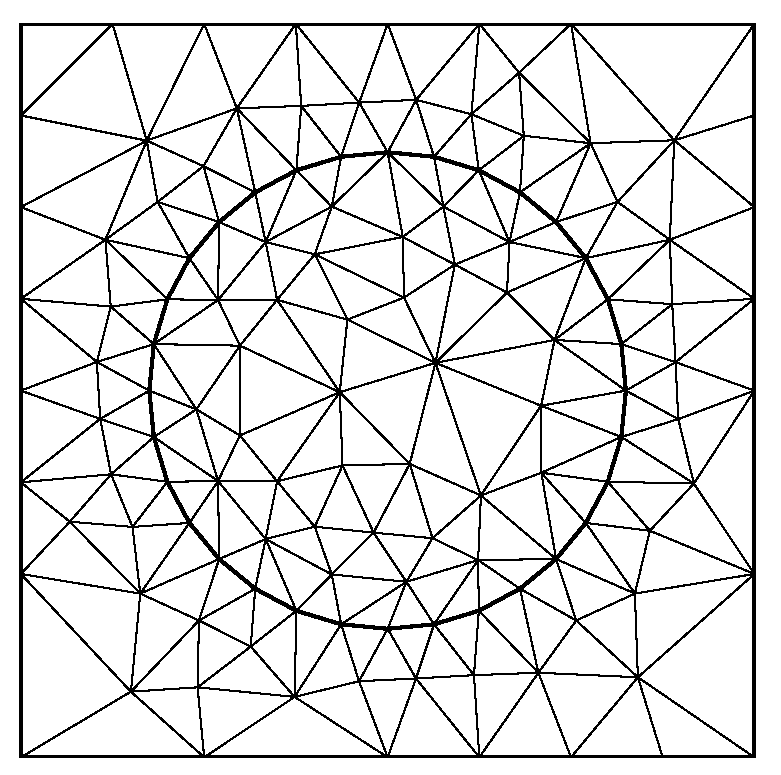
\includegraphics[width=.45\textwidth]
{figures/stokes/fitted_mesh.ps}}
\subfloat[Unfitted mesh]{
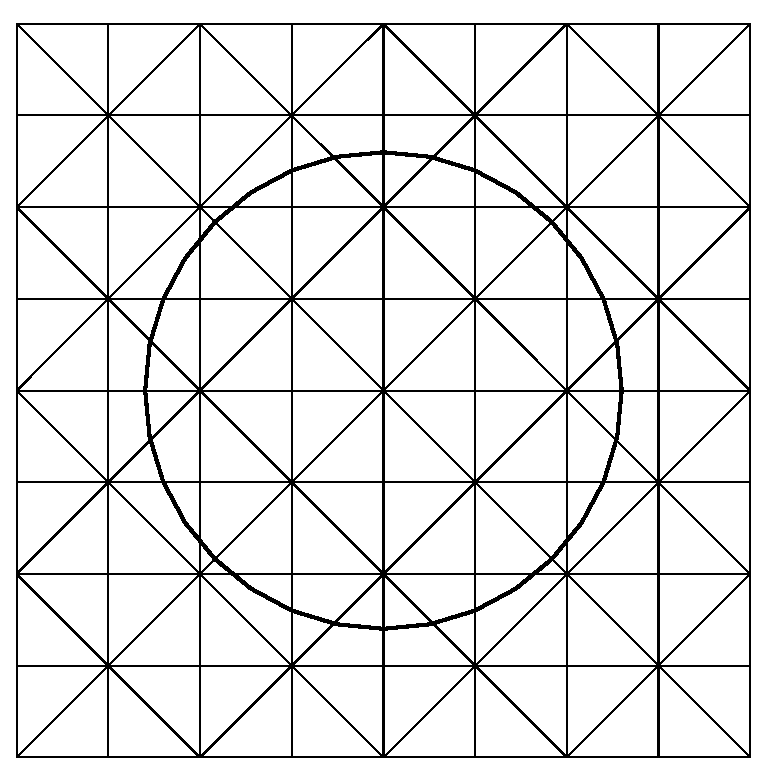
\includegraphics[width=.45\textwidth]
{figures/stokes/unfitted_mesh.ps}}
\caption[Fitted and unfitted meshes]
{Fitted and unfitted meshes for a circular interface.}
\label{fig:fitted_unfitted}
\end{figure}
In the fitted approach, the interface mesh is made up of edges, in 2d, or faces,
in 3d, of elements belonging to the bulk mesh. This means that there is a strong
coupling between the bulk mesh and interface mesh. This is a very intuitive
approach to treat the problem. Discontinuity jumps in the material properties
and in the pressure are captured naturally. In particular, we do not need to
employ an XFEM-type extension of standard bulk pressure spaces. Moreover, there
is no need to transport quantities from the interface to the bulk, or vice
versa. On the other hand, it is not possible to locally refine the bulk mesh
close to the interface without modifying the number of elements of the
interface. Also, every interface deformation corresponds to a bulk deformation,
which means that smoothing and remeshing techniques need to be employed in
order to preserve the bulk mesh quality.

Instead, in the unfitted approach, the interface mesh is completely independent
from the bulk mesh. In particular, there exist bulk elements which are cut by
the interface elements. For this reason there is no need to remesh or deform
the bulk mesh in order to preserve the correspondence with the interface.
Moreover, standard strategies for refinement and coarsening can be employed for
the bulk mesh. Since the bulk mesh is immutable, its quality is preserved
without the need of smoothing techniques. The downside of this approach is that
the quantities computed on the bulk mesh, such as velocity and pressure, need
to be interpolated in order to have their values on the interface. This also
requires finding the intersections between the interface mesh and the bulk mesh
at every time step. Finally, it is necessary to use some XFEM-type extension in
order to capture the discontinuity of quantities of interest across the
interface.

\section{Existence and uniqueness of a discrete solution}
\label{sec:stokes_existence}
\begin{theorem} \label{thm:ex}
Let $m \in \{0,\ldots,M-1\}$ and let $(\uspacedisc{0}{m},\pspace^m)$ satisfy
the LBB condition (\ref{eq:LBB}). Then there exists a unique solution
$(\vec U^{m+1}, P^{m+1}, \vec X^{m+1}, \kappa^{m+1})
\in \uspacedisc{g}{m}\times \pnormspace^m \times \Vh \times \Wh$ to
(\ref{eq:HGa}--d).
\end{theorem}
\begin{proof}
\sloppy As the system (\ref{eq:HGa}--d) is linear, existence follows from
uniqueness. In order to establish the latter, we consider the system: Find
${(\vec U, P, \vec X, \kappa) \in \uspacedisc{0}{m}\times\pnormspace^m \times
\Vh \times \Wh}$ such that
\begin{subequations}
\begin{align}
& 2\left(\mu^m\,\mat D(\vec U), \mat D(\vec \xi) \right)
- \left(P, \nabla\,.\,\vec \xi\right) - \gamma\,\left\langle \kappa\,\vec\nu^m,
\vec\xi\right\rangle_{\Gamma^m} = 0 \quad \forall\ \vec\xi \in
\uspacedisc{0}{m} \,,
\label{eq:proofa}\\
& \left(\nabla\,.\,\vec U, \varphi\right)  = 0 \quad
\forall\ \varphi \in \pnormspace^m\,, \label{eq:proofb} \\
& \left\langle \vec X, \chi\,\vec\nu^m \right\rangle_{\Gamma^m}^h -
\tau_m \left\langle \vec U, \chi\,\vec\nu^m \right\rangle_{\Gamma^m} = 0
\quad\forall\ \chi \in \Wh\,,\label{eq:proofc} \\
& \left\langle \kappa\,\vec\nu^m, \vec\eta \right\rangle_{\Gamma^m}^h
+ \left\langle \nabs\,\vec X, \nabs\,\vec \eta \right\rangle_{\Gamma^m}
= 0  \quad\forall\ \vec\eta \in \Vh\,. \label{eq:proofd}
\end{align}
\end{subequations}
Choosing $\vec\xi=\vec U$ in (\ref{eq:proofa}), $\varphi =  P$ in
(\ref{eq:proofb}), $\chi = \gamma\,\kappa$ in (\ref{eq:proofc}) and
$\vec\eta=\gamma\,\vec X$ in (\ref{eq:proofd}) yields that
\begin{equation}
2\,\tau_m\left(\mu^m\,\mat D(\vec U), \mat D(\vec U) \right)
+ \gamma\,\left\langle \nabs\,\vec X, \nabs\,\vec X \right\rangle_{\Gamma^m}
=0\,, \label{eq:proof2}
\end{equation}
which implies that $\mat D(\vec U) = \mat 0$. We know that the kernel of
$\mat D$ is the space of rigid motions
\begin{equation}\label{eq:rigid_motions_space}
RM=\{\vec \alpha + \mathcal A \vec z:\vec \alpha \in \R^d\,,
\mathcal A \mbox{ antisymmetric matrix in }\R^{d\times d} \}\,,
\end{equation}
see \cite{Mardal2006}. Given that $\vec U \in RM$, in particular we have that
$\vec U(\vec z)$ is linear in $\vec z$. Moreover, $\vec U\in\uspacedisc{0}{m}$
means that $\vec U(\vec z)=\vec 0$ for every corner $\vec z$ of $\Omega$.
Therefore $\vec U(\vec z)=\vec 0$ for all $\vec z\in\Omega$. In addition, it
holds that $\vec X$ is equal to a constant on $\Gamma^m$, which
satisfies, on recalling (\ref{eq:proofc}) and $\vec U = \vec 0$, that
\begin{equation} \label{eq:Xconst}
\left\langle \vec X, \chi\,\vec\nu^m \right\rangle_{\Gamma^m}^h = 0
\quad\forall\ \chi \in \Wh\,.
\end{equation}
It was shown in \cite[Proof of Theorem~2.1]{gflows3d} that if $\Gamma^m$
has no self-intersections, then (\ref{eq:Xconst}) immediately yields that $\vec
X = \vec 0$. As $\Gamma^m = \partial\Omega^m_-$ is the boundary of an open
domain, we always assume that it does not self-intersect, and
hence we obtain that $\vec X = \vec 0$. This means that (\ref{eq:proofd})
reduces to
\begin{equation} \label{eq:kappaproof}
\left\langle \kappa\,\vec\nu^m, \vec\eta \right\rangle_{\Gamma^m}^h = 0
\quad\forall\ \vec\eta \in \Vh\,.
\end{equation}
Let $\vec\omega^m \in \Vh$ be the mass-lumped $L^2$--projection of $\vec\nu^m$
onto $\Vh$, i.e. $\left\langle \vec\omega^m, \vec\varphi
\right\rangle_{\Gamma^m}^h = \left\langle \vec\nu^m,
\vec\varphi \right\rangle_{\Gamma^m}^h = \left\langle \vec\nu^m,
\vec\varphi \right\rangle_{\Gamma^m}$ for all $\vec\varphi\in\Vh$. It is easy
to see that $\vec\omega^m (\vec q^m_k) \not= \vec 0$ for
all $k=1,\ldots,K_\Gamma$, because $\Gamma^m$ does not self-intersect.
Then it follows from choosing $\vec\eta = \vec\omega^m$ in (\ref{eq:kappaproof})
that
\begin{align*}
0 = \left\langle \kappa\,\vec\nu^m, \vec\omega^m \right\rangle_{\Gamma^m}^h
= \left\langle \vec\nu^m, \vec\pi^m[\kappa\,\vec\omega^m]
\right\rangle_{\Gamma^m}
= \left\langle \vec\omega^m,
\vec\pi^m[\kappa\,\vec\omega^m] \right\rangle_{\Gamma^m}^h
= \left\langle \kappa, |\vec\omega^m|^2 \right\rangle_{\Gamma^m}^h ,
\end{align*}
and so $\kappa = 0 \in \Wh$. Finally, it follows from (\ref{eq:proofa}) with
$\vec U = \vec 0$ and $\kappa = 0$, on recalling (\ref{eq:LBB}), that $P = 0$.
Hence there exists a unique solution $(\vec U^{m+1}, P^{m+1}, \vec X^{m+1},$
$\kappa^{m+1}) \in \uspacedisc{g}{m}\times \pnormspace^m \times \Vh \times \Wh$
to (\ref{eq:HGa}--d).
\end{proof}

We note that if $(\uspacedisc{0}{m},\pspace^m)$ does not satisfy the LBB
condition (\ref{eq:LBB}), then existence and uniqueness of the solution
$(\vec U^{m+1},\vec X^{m+1},\kappa^{m+1})$ to a reduced system, where the
pressure $P^{m+1}$ is eliminated, can be shown. More precisely, let
\begin{equation}\label{eq:divfree_u_space}
\uspacesimple^m_0(\vec g) :=
\{ \vec U \in \uspacedisc{g}{m} : (\nabla\,.\,\vec U, \varphi) = 0
\quad \forall \varphi \in \pspace^m \}\,.
\end{equation}
Then any solution $(\vec U^{m+1}, P^{m+1}, \vec X^{m+1}, \kappa^{m+1})
\in \uspacedisc{g}{m}\times \pnormspace^m \times \Vh \times \Wh$
to (\ref{eq:HGa}--d) is such that $(\vec U^{m+1}, \vec X^{m+1}, \kappa^{m+1})
\in \uspacesimple^m_0(\vec g)\times \Vh \times \Wh$ with
\begin{subequations}
\begin{align}
& 2\left(\mu^m\,\mat D(\vec U^{m+1}), \mat D(\vec \xi) \right)
- \gamma\,\left\langle \kappa^{m+1}\,\vec\nu^m,\vec\xi\right\rangle_{\Gamma^m}
= \left(\vec f^{m+1},\vec \xi\right) \quad \forall\ \vec\xi \in
\uspacesimple^m_0(\vec 0)\,, \label{eq:reda}\\
&  \left\langle \frac{\vec X^{m+1} - \vec\id}{\tau_m} ,\chi\,\vec\nu^m
\right\rangle_{\Gamma^m}^h - \left\langle \vec U^{m+1}, \chi\,\vec\nu^m
\right\rangle_{\Gamma^m}  = 0 \quad \forall\ \chi \in \Wh\,,
\label{eq:redb} \\
& \left\langle \kappa^{m+1}\,\vec\nu^m, \vec\eta \right\rangle_{\Gamma^m}^h
+ \left\langle \nabs\,\vec X^{m+1}, \nabs\,\vec \eta \right\rangle_{\Gamma^m} =
0 \quad \forall\ \vec\eta \in \Vh \label{eq:redc}
\end{align}
\end{subequations}

\begin{theorem} \label{thm:stabreduced}
Let $m \in \{0,\ldots,M-1\}$ and let $\uspacesimple^m_0(\vec g)$ be non-empty.
Then there exists a unique solution $(\vec U^{m+1}, \vec X^{m+1}, \kappa^{m+1})
\in \uspacesimple^m_0(\vec g) \times \Vh \times \Wh$ to (\ref{eq:reda}--c).
\end{theorem}
\begin{proof}
As $\uspacesimple^m_0(\vec 0)$ is a subspace of $\uspacedisc{0}{m}$,
existence to the linear system (\ref{eq:reda}--c) follows from uniqueness,
which is easy to show. In fact, similarly to the proof of Theorem~\ref{thm:ex}
we obtain (\ref{eq:proof2}) and hence the desired uniqueness result.
\end{proof}

\section{Stability}\label{sec:stokes_stability}
We now demonstrate that the scheme (\ref{eq:HGa}--d) satisfies an energy
estimate, which corresponds to the bound (\ref{eq:ap1}) in the continuous case.
In particular, we obtain an unconditional stability result for our scheme.

\begin{theorem} \label{thm:stabstab}
\sloppy Let $\vec g=\vec 0$. Moreover let $m \in \{0,\ldots,M-1\}$ and let
${(\vec U^{m+1},P^{m+1},\vec X^{m+1}, \kappa^{m+1}) \in \uspacedisc{0}{m}\times
\pnormspace^m \times \Vh \times \Wh}$ be a solution to (\ref{eq:HGa}--d). Then
\begin{align}\label{eq:stab}
& \gamma\, \surfvol(\Gamma^{m+1})+ 2\,\tau_m\left(\mu^m\,\mat D(\vec U^{m+1}),
\mat D(\vec U^{m+1}) \right) \nonumber \\
& \qquad \leq \gamma\,\surfvol(\Gamma^m) + \tau_m\left( \vec f^{m+1},
\vec U^{m+1} \right).
\end{align}
In addition, let $\{t_k\}_{k=0}^M$ be an arbitrary partitioning of $[0,T]$.

Then it holds that
\begin{align}\label{eq:stabstab}
& \gamma\,\surfvol(\Gamma^{m+1}) + 2 \sum_{k=0}^m  \tau_k\left(\mu^k\,
\mat D(\vec U^{k+1}), \mat D(\vec U^{k+1}) \right) \nonumber \\
& \qquad \leq \gamma\,\surfvol(\Gamma^0) + \sum_{k=0}^m \tau_k\left(\vec
f^{k+1}, \vec U^{k+1} \right)
\end{align}
for $m=0,\ldots, M-1$.
\end{theorem}
\begin{proof}
Choosing $\vec\xi = \vec U^{m+1} \in \uspacedisc{0}{m}$ in (\ref{eq:HGa}),
$\varphi = P^{m+1} \in \pnormspace^m$ in (\ref{eq:HGb}),
$\chi = \gamma\,\kappa^{m+1}$ in (\ref{eq:HGc}) and
$\vec\eta=\gamma\,({\vec X^{m+1}-\vec\id\!\mid_{\Gamma^m}})$ in (\ref{eq:HGd})
yields that
\begin{align*}
& 2\,\tau_m\left(\mu^m\,\mat D(\vec U^{m+1}), \mat D(\vec U^{m+1}) \right)
+ \gamma\,\left\langle \nabs\,\vec X^{m+1}, \nabs\,(\vec X^{m+1} - \vec X^m)
\right\rangle_{\Gamma^m} \nonumber \\
& \qquad = \tau_m\left(\vec f^{m+1}, \vec U^{m+1} \right)\,.
\end{align*}
Hence (\ref{eq:stab}) follows immediately, where we have used
(\ref{eq:delta_length_inequality}). The desired result (\ref{eq:stabstab})
immediately follows from (\ref{eq:stab}).
\end{proof}

\section{Discrete stationary solutions}\label{sec:stokes_stationary_solution}
If the solution $(\vec U^{m+1},P^{m+1},\vec X^{m+1}, \kappa^{m+1})$ to
(\ref{eq:HGa}--d) is such that the interface has not moved,
$\Gamma^{m+1} = \Gamma^m$, then it holds that
\begin{equation}\label{eq:conformal}
\exists\ \zeta \in \Wh \ : \quad \left\langle \zeta\,\vec\nu^m, \vec\eta
\right\rangle_{\Gamma^m}^h + \left\langle \nabs\,\vec \id, \nabs\,\vec \eta
\right\rangle_{\Gamma^m} = 0 \quad \forall\ \vec\eta \in \Vh \,.
\end{equation}
We recall that the proof of Theorem~\ref{thm:equidistribution_property}
shows that
(\ref{eq:conformal}), in the case $d=2$, implies that $\Gamma^m$ is
equidistributed, with the possible exception of elements $\sigma^m_j$ that are
locally parallel to each other; see also \cite[Theorem~2.2]{fdfi}. Moreover, we
recall from \cite[\S4.1]{gflows3d} that surfaces $\Gamma^m \subset \R^3$ that
satisfy (\ref{eq:conformal}) are called conformal polyhedral surfaces.

Next we consider discrete stationary states when no outer forces act, i.e. when
$\vec f = \vec 0$. Here, independently of the choice of $\mu_\pm$, no spurious
velocities appear for discrete stationary solutions. Indeed,
Theorem~\ref{thm:stabstab} has an immediate consequence.
\begin{theorem}\label{thm:stat1}
Let $\vec g=\vec 0$. Let $(\vec U^{m+1},P^{m+1},\vec X^{m+1}, \kappa^{m+1})
\in \uspacedisc{0}{m}\times
\pnormspace^m \times \Vh \times \Wh$ be a solution to  (\ref{eq:HGa}--d) with
$\vec f^{m+1} = \vec 0$. If $\vec X^{m+1} = \vec X^m$, then $\vec U^{m+1} = \vec
0$.
\end{theorem}
\begin{proof}
The solution $(\vec U^{m+1}, \vec X^{m+1})$ fulfils (\ref{eq:stab}) with
$\Gamma^{m+1}$ replaced by $\Gamma^m$ and  $\vec f^{m+1} = \vec 0$. Hence we
obtain $(\mu^m\,\mat D (\vec U^{m+1}), \mat D(\vec U^{m+1})) = 0$ which implies
$\mat D(\vec U^{m+1}) = \mat 0$. Therefore, as shown in the proof of
Theorem~\ref{thm:ex}, it implies $\vec U^{m+1} = \vec 0$.
\end{proof}

Finally, it holds that polyhedral surfaces with constant discrete mean
curvature and zero velocity are stationary solutions
\begin{theorem} \label{thm:stat2}
Let $\vec g=\vec 0$. Let $(\uspacedisc{0}{m},\pspace^m)$ satisfy the LBB
condition (\ref{eq:LBB}) and let
$\charfcn{\Omega^m_-}\in\pspace^m$. Let $\vec f^{m+1} = \vec 0$. Moreover, let
$\Gamma^m$ be a polyhedral surface with constant discrete mean curvature,
i.e. there exists a constant $\overline{\kappa}\in\R$ such that
\begin{equation}\label{eq:constcurv}
\overline{\kappa} \left\langle\vec\nu^m,\vec\eta\right\rangle_{\Gamma^m}
+ \left\langle \nabs\, \vec\id,\nabs\ \vec\eta\right\rangle_{\Gamma^m}=0\quad
\forall \,\vec\eta\in\Vh\,.
\end{equation}
Then $\Gamma^m$ satisfies (\ref{eq:conformal}) and
\begin{equation} \label{eq:solsol}
(\vec U^{m+1}, P^{m+1}, \vec X^{m+1}, \kappa^{m+1}) =
(\vec 0, -\gamma\,\overline\kappa\left[
\charfcn{\Omega_-^m} - \frac{\vol(\Omega_-^m)}{\vol(\Omega)}
\right], \vec\id\!\mid_{\Gamma^m}, \overline{\kappa})
\end{equation}
is the unique solution to (\ref{eq:HGa}--d).
\end{theorem}
\begin{proof}
It immediately follows from (\ref{eq:constcurv}) that (\ref{eq:conformal})
holds. We now show that the solution stated in (\ref{eq:solsol}) solves
(\ref{eq:HGa}--d). Since $\charfcn{\Omega_-^m} \in \pspace^m$, we have
that $P^{m+1} \in \pnormspace^m$, and so (\ref{eq:solsol}) is admissible.
Clearly, the three equations (\ref{eq:HGb}), (\ref{eq:HGc}) and (\ref{eq:HGd})
hold trivially. In order to show that (\ref{eq:HGa}) holds, we observe that the
divergence theorem implies that
\begin{equation*}
- \gamma \left\langle \kappa^{m+1}\,\vec\nu^m, \vec\xi
\right\rangle_{\Gamma^m}
= - \gamma\,\overline\kappa \left\langle \vec\nu^m, \vec\xi
\right\rangle_{\Gamma^m}
= - \gamma\,\overline\kappa \left(\nabla\,.\,\vec\xi,
\charfcn{\Omega_-^m}\right)
= \left(\nabla\,.\,\vec\xi, P^{m+1} \right)
\end{equation*}
for all $\vec\xi \in \uspacedisc{0}{m}$, where we have observed that $P^{m+1}$
differs from $- \gamma\,\overline\kappa\,\charfcn{\Omega_-^m}$ only by a
constant. Hence (\ref{eq:HGa}) also holds, and so (\ref{eq:solsol}) is the
unique solution to (\ref{eq:HGa}--d)
\end{proof}

A stationary solution to the continuous problem with $\vec f = \vec 0$ is a
circle, $d=2$, or a sphere, $d=3$, with zero velocity and a piecewise constant
pressure with a discontinuity across the interface, see (\ref{eq:radialr}--b).

For $d=2$, one can choose $\Gamma^m$ with equidistributed points on a circle as
an approximation of this circle, i.e. a closed regular polygon.
Such a $\Gamma^m$ has constant discrete curvature, i.e. there exists a
$\overline{\kappa} \in \R$ such that (\ref{eq:constcurv}) is satisfied.
Hence Theorem~\ref{thm:stat2} yields that in this situation $(\vec
U^{m+1}, \vec X^{m+1}, \kappa^{m+1}) = (\vec 0, \vec X^m,\overline{\kappa})$ is
the unique solution to the reduced system with $\vec f^{m+1} =\vec 0$. See
\S\ref{sec:stokes_2d_convergence_results} for details.

For $d=3$, we observe in practice that conformal approximations of the sphere,
i.e. spherical $\Gamma^m$ satisfying (\ref{eq:conformal}), also satisfy
(\ref{eq:constcurv}). See \S\ref{sec:stokes_3d_convergence_results} for details.

\section{Semidiscrete scheme}\label{sec:stokes_semi_fem}
We briefly investigate a semidiscrete variant of the scheme (\ref{eq:HGa}--d)
in order to highlight two additional important properties of the scheme: a
good tangential distribution of mesh points, and good volume conservation. For
simplicity, we assume $\vec g=\vec 0$ throughout this section.

Consistently with \S\ref{sec:geometric_pdes_semi_fem}, let
$(\Gamma^h(t))_{t\in[0,T]}$ be a family of polyhedral surfaces, with
outer normal $\vec\nu^h(t)$. We also define the piecewise linear finite element
spaces $\Wht$ and $\Vht$, with $\{\chi^h_k(\cdot,t)\}_{k=1}^{K_\Gamma}$
denoting the standard basis of the former. Hence $\chi^h_k(\vec q^h_l(t),t) =
\delta_{kl}$ for all $k,l \in \{1,\ldots,K_\Gamma\}$ and $t \in [0,T]$, where
$\{\vec q^h_k(t)\}_{k=1}^{K_\Gamma}$ are the vertices of $\Gamma^h(t)$.
We also recall the discrete velocity
\begin{equation*}
\V^h(\vec z, t):=
\sum_{k=1}^{K_\Gamma}\left[\ddt\,\vec q^h_k(t)\right] \chi^h_k(\vec z, t)
\in \Vht\,.
\end{equation*}
For $t\in [0,T]$, let $\mathcal{T}^h(t)$ be a regular partitioning of $\Omega$
into disjoint open simplices and define the finite element spaces $S^h_k(t)$,
$\uspacesimple^h(t)$ and $\pspace^h(t)$ similarly to $S^m_k$,
$\uspacedisc{0}{m}$ and $\pspace^m$, with the corresponding interpolation
operators $I^h_k$ and discrete approximations $\mu^h(t) \in S^h_0(t)$. Here we
recall that we assume $\charfcn{\Omega^h_-(t)}\in\pspace^h(t)$. Then, given
$\Gamma^h(0)$, for $t\in (0,T]$ find $\Gamma^h(t)$ and $(\vec U^h(t), P^h(t),
\V^h(t), \kappa^h(t)) \in \uspacesimple^h(t) \times \pnormspace^h(t) \times
\Vht \times \Wht$ such that
\begin{subequations}
\begin{align}
& 2\left(\mu^h\,\mat D(\vec U^h), \mat D(\vec \xi) \right)
- \left(P^h, \nabla\,.\,\vec \xi\right) - \gamma\,\left\langle
\kappa^h\,\vec\nu^h, \vec\xi\right\rangle_{\Gamma^h(t)} = \left(\vec f^h, \vec
\xi\right) \forall\ \vec\xi \in \uspacesimple^h(t) \,, \label{eq:sda}\\
& \left(\nabla\,.\,\vec U^h, \varphi\right)  = 0
\quad \forall\ \varphi \in \pnormspace^h(t)\,, \label{eq:sdb} \\
& \left\langle \V^h , \chi\,\vec\nu^h
\right\rangle_{\Gamma^h(t)}^h - \left\langle \vec U^h, \chi\,\vec\nu^h
\right\rangle_{\Gamma^h(t)} = 0 \quad \forall\ \chi \in \Wht\,, \label{eq:sdc}
\\
& \left\langle \kappa^h\,\vec\nu^h, \vec\eta \right\rangle_{\Gamma^h(t)}^h
+ \left\langle \nabs\,\vec\id, \nabs\,\vec \eta \right\rangle_{\Gamma^h(t)} = 0
\quad \forall\ \vec\eta \in \Vht\,, \label{eq:sdd}
\end{align}
\end{subequations}
where $\vec f^h := \vec I^h_2\,\vec f(t)$.

First of all we note that a solution $\Gamma^h(t)$ to (\ref{eq:sda}--d) clearly
satisfies (\ref{eq:conformal}), with $\Gamma^m$ replaced by $\Gamma^h(t)$. This
means that in 2d the polygonal curve $\Gamma^h(t)$ is equidistributed, and
asymptotically this property is inherited by our fully discrete scheme
(\ref{eq:HGa}--d); see e.g. Figure~\ref{fig:nonuniform_bubble_32_both} below.
In 3d the property (\ref{eq:conformal}) means that $\Gamma^h(t)$ is a
conformal polyhedral surface, which implies that the mesh quality is good. Once
again, we observe in practice that the fully discrete solutions to
(\ref{eq:HGa}--d) also exhibit nice meshes, without coalescence or other
mesh defects occurring.

Secondly, we can show that solutions to (\ref{eq:sda}--d) satisfy a discrete
analogue of (\ref{eq:conserved}). To see this, choose $\chi = 1$ in
(\ref{eq:sdc}) and $\varphi= (\charfcn{\Omega_-^h(t)} -
\frac{\vol(\Omega_-^h(t))}{\vol(\Omega)})
\in \pnormspace^h(t)$ in (\ref{eq:sdb}), to obtain
\begin{align}\label{eq:stokes_volume_semidiscrete}
\ddt \vol(\Omega_-^h(t))  &=
\left\langle \V^h , \vec\nu^h \right\rangle_{\Gamma^h(t)}
= \left\langle \V^h , \vec\nu^h \right\rangle^h_{\Gamma^h(t)}
= \left\langle \vec U^h, \vec\nu^h \right\rangle_{\Gamma^h(t)} \nonumber \\
&= \int_{\Omega_-^h(t)} \nabla\,.\,\vec U^h \dL{d} =
\left(\nabla\,.\,\vec U^h , \charfcn{\Omega_-^h(t)}\right) \nonumber \\
&=\left(\nabla\,.\,\vec U^h , \charfcn{\Omega_-^h(t)}\right) -
\frac{\vol(\Omega_-^h(t))}{\vol(\Omega)}\,\left(\nabla\,.\,\vec U^h , 1 \right)
= 0\,,
\end{align}
given that
\begin{equation}
\left(\nabla\,.\,\vec U^h , 1 \right)
= \int_{\partial\Omega} \vec U^h\,.\,\unitn\dH{d-1} = 0\,.
\end{equation}
Hence solution to (\ref{eq:sda}--d) conserve the enclosed volume. Once again,
the fully discrete scheme (\ref{eq:HGa}--d) inherits this property in the sense
that in our simulations the volumes are always well maintained, with the
observed relative volume loss tending to zero as $\tau\to 0$.

\section{Algebraic formulation}\label{sec:stokes_algebraic_system}
As is standard practice for the solution of linear systems arising from
discretizations of (Navier--)Stokes equations, we avoid the complications of the
constrained pressure space $\pnormspace^m$ in practice by considering an
overdetermined linear system with $\pspace^m$ instead. In a post-processing step
the computed pressure is then projected into the space of zero mean
functions. The adoption of the unconstrained pressure space $\pspace^m$
requires particular care when the Dirichlet boundary data $\vec g$ is different
from zero. Indeed, let $\varphi \in \pspace^m$, then we can rewrite $\varphi$ as
\begin{equation}\label{eq:phi_rewriting}
\varphi=\varphi-\frac{\left(\varphi,1\right)}{\left(1,1\right)}
+\frac{\left(\varphi,1\right)}{\left(1,1\right)}\,,
\end{equation}
where $\varphi-\frac{(\varphi,1)}{(1,1)}\in\pnormspace^m$ and
$\frac{(\varphi,1)}{(1,1)}\in\R$. Substituting (\ref{eq:phi_rewriting}) in
(\ref{eq:HGb}) we obtain
\begin{equation}
\left(\nabla\,.\,\vec U^{m+1}, \varphi\right)  =
\left(\nabla\,.\,\vec U^{m+1},
\varphi-\frac{\left(\varphi,1\right)}{\left(1,1\right)}\right) +
\left(\nabla\,.\,\vec U^{m+1},1\right)
\frac{\left(\varphi,1\right)}{\left(1,1\right)}\,,
\end{equation}
but, from (\ref{eq:HGb}), we have
\begin{equation}
\left(\nabla\,.\,\vec U^{m+1},
\varphi-\frac{\left(\varphi,1\right)}{\left(1,1\right)}\right) = 0\,,
\end{equation}
and, noting that
\begin{equation}\label{eq:div_to_line_integral}
\left(\nabla\,.\,\vec U^{m+1}, 1\right)=
\int_{\partial\Omega}\vec U^{m+1}\,.\, \unitn \dH{d-1}=
\int_{\partial_1\Omega}(\vec I^m_2\,\vec g) \,.\, \unitn \dH{d-1}\,,
\end{equation}
we finally deduce
\begin{equation} \label{eq:LAb}
 \left(\nabla\,.\,\vec U^{m+1}, \varphi\right) =
 \frac{\left(\varphi, 1\right)}{\vol(\Omega)}\, \int_{\partial_1\Omega}
(\vec I^m_2\,\vec g) \,.\, \unitn \dH{d-1} \quad \forall\ \varphi \in
\pspace^m\,.
\end{equation}
Therefore, as in our case, when the pressure space used is the unconstrained
space $\pspace^m$ instead of $\pnormspace^m$, then the equation (\ref{eq:LAb})
replaces (\ref{eq:HGb}) and the resulting finite element approximation is: For
$m=0,\ldots, M-1$, find ${(\vec U^{m+1}, P^{m+1}, \vec X^{m+1}, \kappa^{m+1})
\in \uspacedisc{g}{m}\times \pspace^m \times \Vh \times \Wh}$ such that
\begin{subequations}
\begin{align}
& 2\left(\mu^m\,\mat D(\vec U^{m+1}), \mat D(\vec \xi) \right)
- \left(P^{m+1}, \nabla\,.\,\vec \xi\right) \nonumber \\
& \qquad - \gamma\,\left\langle
\kappa^{m+1}\,\vec\nu^m,\vec\xi\right\rangle_{\Gamma^m}
= \left(\vec f^{m+1},\vec \xi\right) \quad \forall\ \vec\xi \in
\uspacedisc{0}{m}\,, \label{eq:HGcorrecteda}\\
& \left(\nabla\,.\,\vec U^{m+1}, \varphi\right)  =
\frac{\left(\varphi, 1\right)}{\vol(\Omega)}\, \int_{\partial_1\Omega}
(\vec I^m_2\,\vec g) \,.\, \unitn \dH{d-1}
\quad \forall\ \varphi \in \pspace^m\,,\label{eq:HGcorrectedb} \\
&  \left\langle \frac{\vec X^{m+1} - \vec\id}{\tau_m} ,\chi\,\vec\nu^m
\right\rangle_{\Gamma^m}^h - \left\langle \vec U^{m+1}, \chi\,\vec\nu^m
\right\rangle_{\Gamma^m}  = 0 \quad \forall\ \chi \in \Wh\,,
\label{eq:HGcorrectedc} \\
& \left\langle \kappa^{m+1}\,\vec\nu^m, \vec\eta \right\rangle_{\Gamma^m}^h
+ \left\langle \nabs\,\vec X^{m+1}, \nabs\,\vec \eta \right\rangle_{\Gamma^m} =
0 \quad \forall\ \vec\eta \in \Vh \label{eq:HGcorrectedd}
\end{align}
\end{subequations}
and set $\Gamma^{m+1} = \vec X^{m+1}(\Gamma^m)$.

Let $\uspacesimple^m$ be the unconstrained velocity space, with basis
$\{\phi_i^{\uspacesimple^m}\}_{i=1}^{K^m_\uspacesimple}$. Moreover, let
$\{\phi_i^{\pspace^m}\}_{i=1}^{K^m_\pspace}$ span the unconstrained pressure
space $\pspace^m$ and let $\{\chi_i^m\}_{i=1}^{K_\Gamma}$ be the basis of
$\Wh$. Then, ignoring for now the Dirichlet and free-slip boundary conditions,
the resulting linear system can be formulated as: Find ${(\vec U^{m+1},P^{m+1},
\kappa^{m+1},\delta\vec X^{m+1})\in (\R^d)^{K^m_\uspacesimple}\times
\R^{K^m_\pspace} \times \R^{K_\Gamma}\,\times (\R^d)^{K_\Gamma}}$, where $\vec
X^{m+1} = \vec X^m+ \delta\vec X^{m+1}$, such that
\begin{equation}
\begin{pmatrix}
\vec B_\Omega & \vec C_\Omega & -\gamma\,\Nbulk & 0 \\
\vec C^T_\Omega & 0 & 0 & 0 \\
\NbulkT & 0 & 0 & -\frac1{\tau_m}\,\vec N_\Gamma^T \\
0 & 0 & \vec N_\Gamma & \vec A_\Gamma
\end{pmatrix}
\begin{pmatrix}
\vec U^{m+1} \\
P^{m+1} \\
\kappa^{m+1} \\
\delta\vec X^{m+1}
\end{pmatrix}
=
\begin{pmatrix}
\vec c \\
\vec \beta \\
0 \\
-\vec A_\Gamma\,\vec X^m
\end{pmatrix} \,,
\label{eq:stokes_algebraic}
\end{equation}
where $(\vec U^{m+1},P^{m+1},\kappa^{m+1},\delta\vec X^{m+1})$ here denote the
coefficients of these finite element functions with respect to the
aforementioned (basis) functions.
Moreover, $\vec X^m$ denotes the coefficients of
$\vec\id\!\mid_{\Gamma^m}$ with respect to the basis of $\Vh$. The definitions
of the matrices and vectors in (\ref{eq:stokes_algebraic}) directly follow from
(\ref{eq:HGcorrecteda}--d) and are:
\begin{align*}
& [\vec B_\Omega]_{ij} := 2\left(\left(\mu^m\,\mat D(\phi_j^{\uspacesimple^m}
\vec e_q), \mat D( \phi_i^{\uspacesimple^m}\,\vec e_r) \right)
\right)_{q,r=1}^d\,,\quad
\vec c_i := \left( \vec f^{m+1},\phi_i^{\uspacesimple^m}\right)\,,\\
&[\vec C_\Omega]_{ip} := - \left(
\left(\nabla\,.\,(\phi_i^{\uspacesimple^m}\,\vec
e_q), \phi_p^{\pspace^m} \right) \right)_{q=1}^d,\quad
[\Nbulk]_{il} := \left\langle \phi_i^{\uspacesimple^m}, \chi^m_l \,\vec\nu^m
\right\rangle_{\Gamma^m} \,,\\
& \vec \beta_i := \frac{\left(\phi_i^{\pspace^m},1\right)}{\left(1,1\right)}
\left\langle \vec I_2^m\,\vec g,\unitn\right\rangle_{\partial_1\Omega}\,,\quad
[\vec N_\Gamma]_{kl} := \left\langle \chi^m_l, \chi^m_k\,\vec\nu^m
\right\rangle_{\Gamma^m}^h \,,\\
& [\vec A_\Gamma]_{kl} := \left\langle \nabs\,\chi^m_l, \nabs\,\chi^m_k
\right\rangle_{\Gamma^m} \,\vec\id \,,
\end{align*}
where $\{\vec e_q\}_{q=1}^d$ denotes the standard basis in $\R^d$. Note that
for the submatrices we have used the convention that the subscripts refer to
the test and trial domains, respectively. A single subscript is used where the
two domains are the same.

The Dirichlet boundary condition can be imposed by doctoring the matrix and the
right-hand side of the algebraic system (\ref{eq:stokes_algebraic}). The matrix
doctoring process consists on zeroing the rows which correspond to the Dirichlet
boundary degrees of freedom in $\vec B_\Omega$, $\vec C_\Omega$ and $\Nbulk$ in
the first block row of (\ref{eq:stokes_algebraic}) and setting a unitary value
on the correspondent diagonal entries in $\vec B_\Omega$. The vector doctoring
process consists on setting the Dirichlet boundary data on the correspondent
right-hand side entries in $\vec c$. Similarly, the free-slip boundary
condition is enforced by doctoring the matrix entries corresponding to
the degrees of freedom of the basis functions
$\phi_i^{\uspacesimple^m}\vec e_q$ associated with vertices that lie on
parts of $\partial_2\Omega$ that satisfy $\vec e_q=\unitn$. Of course,
the corresponding entries in the right-hand side vector $\vec c$ are set to
zero.

We observe the analogy of the interface part of the algebraic system,
namely the matrices $[\vec A_\Gamma]$ and $[\vec N_\Gamma]$ and the right-hand
side term $-\vec A_\Gamma\,\vec X^m$, with the algebraic system arising
from the mean curvature flow (\ref{eq:algebraic_mean_curvature}) and surface
diffusion (\ref{eq:algebraic_surf_diff}).

\section{Solution method}\label{sec:stokes_solution_method}
For the solution of (\ref{eq:stokes_algebraic}) we use a Schur complement
approach that eliminates $(\kappa^{m+1}, \delta \vec X^{m+1})$ from
(\ref{eq:stokes_algebraic}), and then use an iterative solver for the remaining
system in $(\vec U^{m+1}, P^{m+1})$. This approach has the advantage that for
the reduced system well-known solution methods for finite element
discretizations for standard (Navier--)Stokes discretizations may be employed.
The desired Schur complement can be obtained as follows. Let
\begin{equation} \label{eq:Xi}
\Xi_\Gamma:= \begin{pmatrix}
 0 & - \frac1{\tau_m}\,\vec N_\Gamma^T \\
\vec N_\Gamma & \vec A_\Gamma
\end{pmatrix} \,,
\end{equation}
be the interface condensed operator, which is exactly the same operator
(\ref{eq:algebraic_initial_curvature}) arising from the discretization of the
stationary geometric PDE. Then (\ref{eq:stokes_algebraic}) can be reduced to
\begin{subequations}
\begin{align}\label{eq:SchurkX}
&
\begin{pmatrix}
\vec B_\Omega + \gamma\,(\Nbulk \ 0)\,\Xi_\Gamma^{-1}\,
\binom{\NbulkT}{0} & \vec C_\Omega \\
\vec C_\Omega^T & 0
\end{pmatrix}
\begin{pmatrix}
\vec U^{m+1} \\ P^{m+1}
\end{pmatrix}
= \nonumber \\
& \qquad
\begin{pmatrix}
\vec c
+\gamma\,(\Nbulk \ 0)\, \Xi_\Gamma^{-1}\,
\binom{0}{-\vec A_\Gamma\,\vec X^m} \\
\vec \beta
\end{pmatrix}
\end{align}
and
\begin{equation}
\binom{\kappa^{m+1}}{\delta\vec X^{m+1}} = \Xi_\Gamma^{-1}\,
\binom{-\NbulkT\,\vec U^{m+1}}{-\vec A_\Gamma\,\vec X^m}\,.
\label{eq:SchurkXb}
\end{equation}
\end{subequations}

We notice that when $\gamma = 0$ the linear system (\ref{eq:SchurkX}) becomes
\begin{equation} \label{eq:stokes_system}
\begin{pmatrix}
\vec B_\Omega & \vec C_\Omega \\
\vec C_\Omega^T & 0
\end{pmatrix}
\begin{pmatrix}
\vec U^{m+1} \\ P^{m+1}
\end{pmatrix}
= \begin{pmatrix}
\vec c \\
\vec \beta
\end{pmatrix}\,,
\end{equation}
which for $\mu_+=\mu_-$ corresponds to a discretization of the one-phase
Stokes problem. This system is well known and a classical way to solve it is to
use a preconditioned GMRES iteration. The generalized minimal residual method
(GMRES) is an iterative method for non-symmetric systems. It generates a
sequence of orthogonal vectors using the Arnoldi method which is a modified
Gram-Schmidt orthogonalization applied to a Krylov subspace with minimal
residual. See \cite{BarrettBCetal94} for more details. Therefore, we solve
(\ref{eq:SchurkX}), which is a slight modification of (\ref{eq:stokes_system}),
employing a preconditioned GMRES iterative solver. For the inverse
$\Xi_\Gamma^{-1}$ we employ a sparse $L\,U$ decomposition, which we obtain with
the help of the sparse factorization package UMFPACK, see \cite{Davis04}, in
order to reuse the factorization. Having obtained $(\vec U^{m+1}, P^{m+1})$ from
(\ref{eq:SchurkX}), we solve (\ref{eq:SchurkXb}) for $(\kappa^{m+1}, \delta\vec
X^{m+1})$.

As regarding the preconditioner, see \cite{ElmanSW05} for more details, a
possible choice is to use the preconditioner
\begin{equation} \label{eq:ESW}
\mathcal{P} = \begin{pmatrix}
\vec{\mathcal{P}}_{\vec B} & \vec C_\Omega \\
0 & -\mathcal{P}_S
\end{pmatrix}\,,
\end{equation}
where $\vec{\mathcal{P}}_{\vec B}$ is some preconditioner for the matrix $\vec
B_\Omega$, and $\mathcal{P}_S$ acts as a preconditioner for the bulk Schur
complement operator $S_\Omega=\vec C^T_\Omega \,\vec B_\Omega^{-1}\,\vec
C_\Omega$.

An application of the preconditioner (\ref{eq:ESW}) amounts to solving the
equations
\begin{equation*}
\begin{pmatrix}
\vec{\mathcal{P}}_{\vec B} & \vec C_\Omega \\
0 & -\mathcal{P}_S
\end{pmatrix}
\begin{pmatrix} \vec U \\ P \end{pmatrix}
= \begin{pmatrix} \vec v \\ q \end{pmatrix}
\end{equation*}
which, by backward substitution, is equivalent to
\begin{equation}\label{eq:blocksolution}
\mathcal{P}_S\,P = -q\,,\quad \vec{\mathcal{P}}_{\vec B}\,\vec U = \vec v -
\vec C_\Omega\,P\,.
\end{equation}
We choose $\vec B_\Omega$  for $\vec{\mathcal{P}}_{\vec B}$ and the pressure
mass matrix $M_\Omega$ defined as
\begin{equation*}
[M_\Omega]_{ij} = \left(\,\phi_j^{\pspace^m},\, \phi_i^{\pspace^m}\right)\,.
\end{equation*}
for $\mathcal{P}_S$. Again, in order to reuse the factorization, we employ a
sparse $L\,U$ decomposition to factorize the matrices $\vec B$ and $M_\Omega$.

Alternatively, it is possible to use the standard Stokes matrix, see
(\ref{eq:stokes_system}),
\begin{equation}\label{eq:stokes_direct_precond}
\begin{pmatrix}
\vec B_\Omega & \vec C_\Omega \\
\vec C_\Omega^T & 0
\end{pmatrix}\,
\end{equation}
as a preconditioner for (\ref{eq:SchurkX}) and factorize it directly with a
sparse $L\,U$ decomposition. Since in the Stokes problem the pressure
solution is only unique up to a constant, the matrix
(\ref{eq:stokes_direct_precond}) is singular. In particular, if LBB holds, the
matrix has rank deficiency 1. Therefore, in order to use UMFPACK to factorize
the matrix, the rank deficiency needs to be reduced to 0. This can be achieved
by fixing a degree of freedom in the discrete pressure. For example, by
using a matrix doctoring which replaces the first row of the second block row
of (\ref{eq:stokes_direct_precond}) with the corresponding row of the identity
matrix. This doctoring
process can be avoided if SPQR is used to factorize the preconditioner since
SPQR can decompose also singular matrices. Indeed, SPQR is a sparse
factorization package, see \cite{Davis11}, performing a QR decomposition which
can be used to solve the least squares problem.

The algebraic system (\ref{eq:stokes_algebraic}) can be rewritten when we
use (P1+P0) or \pdg as pressure space. Indeed it assumes the following form
\begin{equation}
\begin{pmatrix}
\vec B_\Omega & \vec C_{\spadesuit} & \vec C_{\clubsuit} & -\gamma\,\Nbulk & 0\\
\vec C^T_{\spadesuit} & 0 & 0 & 0 & 0 \\
\vec C^T_{\clubsuit} & 0 & 0 & 0 & 0 \\
\NbulkT & 0 & 0 & 0 & -\frac1{\tau_m}\,\vec N_\Gamma^T \\
0 & 0 & 0 & \vec N_\Gamma & \vec A_\Gamma
\end{pmatrix}
\begin{pmatrix}
\vec U^{m+1} \\
P^{m+1}_\spadesuit \\
P^{m+1}_\clubsuit \\
\kappa^{m+1} \\
\delta\vec X^{m+1}
\end{pmatrix}
=
\begin{pmatrix}
\vec c \\
\vec \beta_\spadesuit \\
\vec \beta_\clubsuit \\
0 \\
-\vec A_\Gamma\,\vec X^m
\end{pmatrix} \,,
\label{eq:stokes_algebraic_extended}
\end{equation}
where $\vec C_{\spadesuit}$ and $\vec C_{\clubsuit}$ have the same definition
of $\vec C_\Omega$ in (\ref{eq:stokes_algebraic}) but now in terms of bases of
different spaces. More precisely, in the case (P1+P0), there are two
independent spaces for the pressure of polynomial order 1 and 0, respectively.
Instead, in the case \pdg, both spaces have polynomial degree 1 but the basis
functions support is restricted to $\Omega_-^m$ and $\Omega_+^m$, respectively.

A suitable preconditioner for the algebraic system
(\ref{eq:stokes_algebraic_extended}) is then
\begin{equation} \label{eq:ESW_extended}
\mathcal{P} = \begin{pmatrix}
\vec{\mathcal{P}}_{\vec B} & \vec C_\spadesuit & \vec C_\clubsuit \\
0 & -\mathcal{P}_{S,\spadesuit} & 0 \\
0 & 0 &-\mathcal{P}_{S,\clubsuit}
\end{pmatrix}\,,
\end{equation}
while the reduced system (\ref{eq:SchurkX}) becomes
\begin{align}\label{eq:SchurkX_extended}
&
\begin{pmatrix}
\vec B_\Omega + \gamma\,(\Nbulk \ 0)\,\Xi_\Gamma^{-1}\,\binom{\NbulkT}{0} &
\vec C_\spadesuit & \vec C_\clubsuit \\
\vec C^T_\spadesuit & 0 & 0 \\
\vec C^T_\clubsuit & 0 & 0 \\
\end{pmatrix}
\begin{pmatrix}
\vec U^{m+1} \\
P^{m+1}_\spadesuit \\
P^{m+1}_\clubsuit
\end{pmatrix}
= \nonumber \\
& \qquad
\begin{pmatrix}
\vec c+\gamma\,(\Nbulk \ 0)\,
\Xi_\Gamma^{-1}\,\binom{0}{-\vec A_\Gamma\,\vec X^m} \\
\vec \beta_\spadesuit \\
\vec \beta_\clubsuit
\end{pmatrix}\,.
\end{align}
An application of the preconditioner (\ref{eq:ESW_extended}) amounts to solving
the equations
\begin{equation*}
\begin{pmatrix}
\vec{\mathcal{P}}_{\vec B} & \vec C_\spadesuit & \vec C_\clubsuit \\
0 & -\mathcal{P}_{S,\spadesuit} & 0 \\
0 & 0 &-\mathcal{P}_{S,\clubsuit}
\end{pmatrix}
\begin{pmatrix}
\vec U \\
P_\spadesuit \\
P_\clubsuit
\end{pmatrix}
=
\begin{pmatrix}
\vec v \\
q \\
p
\end{pmatrix}
\end{equation*}
which, by backward substitution, is equivalent to
\begin{equation}\label{eq:blocksolution_extended}
\mathcal{P}_{S,\spadesuit}\,P_\spadesuit =
-q\,,\quad \mathcal{P}_{S,\clubsuit}\,P_\clubsuit =
-p\,,\quad \vec{\mathcal{P}}_{\vec B}\,\vec U =
\vec v - \vec C_\spadesuit\,P_\spadesuit - \vec C_\clubsuit\,P_\clubsuit\,.
\end{equation}

Alternatively, as before, it is possible to use the standard Stokes matrix
\begin{equation}\label{eq:stokes_direct_precond_extended}
\begin{pmatrix}
\vec B_\Omega & \vec C_\spadesuit & \vec C_\clubsuit \\
\vec C^T_\spadesuit & 0 & 0 \\
\vec C^T_\clubsuit & 0 & 0 \\
\end{pmatrix}
\end{equation}
as a preconditioner for (\ref{eq:SchurkX_extended}) and factorize them directly
with a sparse $L\,U$ decomposition. The matrix
(\ref{eq:stokes_direct_precond_extended}), if LBB holds, has rank deficiency 1
for the P2--\pdg element and 2 for the P2--(P1+P0) element. Therefore, in the
case P2--\pdg, only the block entry in position $(2,2)$ of
(\ref{eq:stokes_direct_precond_extended}) is doctored while, in the case
P2--(P1+P0), the block entries in position in position $(2,2)$ and $(3,3)$ of
(\ref{eq:stokes_direct_precond_extended}) are doctored. Again, we point out
that the doctoring is not needed when SPQR is used to factorize the
preconditioner.

\section{Mesh generation and smoothing}\label{sec:stokes_smoothing}
Given the initial polyhedral surface $\Gamma^0$, we create a triangulation
$\mathcal{T}^0$ of $\Omega$ that is fitted to $\Gamma^0$ with the help of the
package \verb|Gmsh|, see \cite{GeuzaineR09}.

The mesh generation process is controlled by the characteristic lengths of the
points describing the geometry of the domain boundary $\partial\Omega$. Each
point has associated a characteristic length which prescribes the size of the
mesh elements. For example, a segment of length $L$, which defines an edge of
the domain boundary, delimited by two points of characteristic length $c_l$ will
be subdivided into several segments of lengths $\frac{L}{c_l}$ during the mesh
generation. Therefore, the smaller is the characteristic length, the finer is
the resulting mesh. When the characteristic lengths of two points defining an
edge are different, \verb|Gmsh| performs an interpolation process. In general we
use either nearly uniform or adaptive bulk meshes. In the former case, the
characteristic length $c_l$ is set to be equal to the characteristic length of
the interface $c_{l,\Gamma}$, while in the latter case the characteristic
length is $c_l(\vec z)=\min\{8c_{l,\Gamma},\mbox{dist}(\vec z,\Gamma)\}$.
Therefore, in the adaptive case, if the interface is far enough from the
boundary, the resulting bulk mesh will be coarse. We define the characteristic
length of the interface $c_{l,\Gamma}$, in the 2d case, as the average length
of the segments describing the discrete interface $\Gamma^m$ or, in the 3d
case, as the length of an equilateral triangle with area equal to the average
of the areas of the triangles describing the discrete interface $\Gamma^m$.

Then, for $m \geq 0$, having computed the new interface $\Gamma^{m+1}$, we
would like to obtain a bulk triangulation $\mathcal{T}^{m+1}$ that is fitted to
$\Gamma^{m+1}$, and ideally is close to $\mathcal{T}^m$. This is to avoid
unnecessary overhead from remeshing the domain $\Omega$ completely.

To this end, we perform the following smoothing step on $\mathcal{T}^m$, which
is inspired by the method proposed in \cite{Ganesan06}, see also
\cite{GanesanT08}. Having obtained $\delta \vec X^{m+1}$ from the solution of
(\ref{eq:stokes_algebraic}), we solve the linear elasticity problem: Find a
displacement
$\vec\psi \in [H^1(\Omega)]^d$ such that
\begin{subequations}
\begin{alignat}{2}
\nabla\,.\,\mat S & = \vec 0 \quad &&\mbox{in } \Omega_\pm^m\,,
\label{eq:elasta}\\
\vec\psi &= \delta \vec X \quad && \mbox{on } \Gamma^m\,, \label{eq:elastb} \\
\vec\psi\,.\,\unitn & = 0 \quad &&\mbox{on } \partial\Omega\,,
\label{eq:elastc}
\end{alignat}
\end{subequations}
where the stress tensor $\mat S$ is defined as
\begin{equation} \label{eq:elasticity_tensor}
\mat S = 2\,\mat D(\vec\psi) + (\nabla\,.\vec\psi)\,\mat\id\,.
\end{equation}
In practice we approximate (\ref{eq:elasta}--c)
with piecewise linear elements and solve the resulting system of linear
equations with the UMPFACK package, see \cite{Davis04}. The obtained discrete
variant of $\vec\psi$, at every vertex of the current bulk grid
$\mathcal{T}^m$, then represents the variation in their position that we
compute in order to obtain $\mathcal{T}^{m+1}$.

Occasionally the deformation of the mesh becomes too large, for instance when
the bubble making up the inner phase undergoes strong deformations, and so a
complete remeshing of $\Omega$ becomes necessary. In order to detect the need
for a complete remeshing, we define the volume criterion
\begin{equation}\label{eq:volume_criterion}
\frac{\max_{\sigmaO\in {\cal T}^{m+1}}\vol(\sigmaO)}
{\min_{\sigmaO\in\mathcal {T}^{m+1}}\vol(\sigmaO)} \geq C_v \geq 1,
\end{equation}
where $C_v$ is a fixed constant. Of course, if we choose $C_v = 1$, then a
remeshing would be triggered after every time step, while, if we choose $C_v =
\infty$, then no remeshing would ever be triggered. Obviously, the
volume criterion (\ref{eq:volume_criterion}) cannot be used for adaptive
meshes therefore we also define the angle criterion
\begin{equation}\label{eq:angle_criterion}
\min_{\sigmaO\in {\cal T}^{m+1}}\min_{\alpha\in \measuredangle(\sigmaO)}\alpha
\leq C_a\,,
\end{equation}
where $\measuredangle(\sigmaO)$ is the set of all the angles of the simplex
$\sigmaO$ which can be computed as $\alpha_{ij}=\cos^{-1}(-\vec n_i\,.\,\vec
n_j)$, $\forall i,j\in\{0,\dots,d\}$, with $\vec n_i$ the unitary normal to the
simplex face $i$. Of course, if we chose $C_a=60$\textdegree, then a remeshing
is triggered after every time step, while, if we choose
$C_a = 0$\textdegree, then no remeshing would ever be triggered.

We stress that in all our numerical simulations we never need to remesh the
interface $\Gamma^m$ itself. Hence the stability results from
Theorem~\ref{thm:stabstab} hold throughout. Of course, a remeshing of $\Gamma^m$
would mean that (\ref{eq:stab}) in Theorem~\ref{thm:stabstab} is no longer
valid because the re-meshed interface $\hat{\Gamma}^m$ differs from the
computed $\Gamma^m$.
